% Template for PLoS
% Version 3.5 March 2018
%
% % % % % % % % % % % % % % % % % % % % % %
%
% -- IMPORTANT NOTE
%
% This template contains comments intended 
% to minimize problems and delays during our production 
% process. Please follow the template instructions
% whenever possible.
%
% % % % % % % % % % % % % % % % % % % % % % % 
%
% Once your paper is accepted for publication, 
% PLEASE REMOVE ALL TRACKED CHANGES in this file 
% and leave only the final text of your manuscript. 
% PLOS recommends the use of latexdiff to track changes during review, as this will help to maintain a clean tex file.
% Visit https://www.ctan.org/pkg/latexdiff?lang=en for info or contact us at latex@plos.org.
%
%
% There are no restrictions on package use within the LaTeX files except that 
% no packages listed in the template may be deleted.
%
% Please do not include colors or graphics in the text.
%
% The manuscript LaTeX source should be contained within a single file (do not use \input, \externaldocument, or similar commands).
%
% % % % % % % % % % % % % % % % % % % % % % %
%
% -- FIGURES AND TABLES
%
% Please include tables/figure captions directly after the paragraph where they are first cited in the text.
%
% DO NOT INCLUDE GRAPHICS IN YOUR MANUSCRIPT
% - Figures should be uploaded separately from your manuscript file. 
% - Figures generated using LaTeX should be extracted and removed from the PDF before submission. 
% - Figures containing multiple panels/subfigures must be combined into one image file before submission.
% For figure citations, please use "Fig" instead of "Figure".
% See http://journals.plos.org/plosone/s/figures for PLOS figure guidelines.
%
% Tables should be cell-based and may not contain:
% - spacing/line breaks within cells to alter layout or alignment
% - do not nest tabular environments (no tabular environments within tabular environments)
% - no graphics or colored text (cell background color/shading OK)
% See http://journals.plos.org/plosone/s/tables for table guidelines.
%
% For tables that exceed the width of the text column, use the adjustwidth environment as illustrated in the example table in text below.
%
% % % % % % % % % % % % % % % % % % % % % % % %
%
% -- EQUATIONS, MATH SYMBOLS, SUBSCRIPTS, AND SUPERSCRIPTS
%
% IMPORTANT
% Below are a few tips to help format your equations and other special characters according to our specifications. For more tips to help reduce the possibility of formatting errors during conversion, please see our LaTeX guidelines at http://journals.plos.org/plosone/s/latex
%
% For inline equations, please be sure to include all portions of an equation in the math environment.  For example, x$^2$ is incorrect; this should be formatted as $x^2$ (or $\mathrm{x}^2$ if the romanized font is desired).
%
% Do not include text that is not math in the math environment. For example, CO2 should be written as CO\textsubscript{2} instead of CO$_2$.
%
% Please add line breaks to long display equations when possible in order to fit size of the column. 
%
% For inline equations, please do not include punctuation (commas, etc) within the math environment unless this is part of the equation.
%
% When adding superscript or subscripts outside of brackets/braces, please group using {}.  For example, change "[U(D,E,\gamma)]^2" to "{[U(D,E,\gamma)]}^2". 
%
% Do not use \cal for caligraphic font.  Instead, use \mathcal{}
%
% % % % % % % % % % % % % % % % % % % % % % % % 
%
% Please contact latex@plos.org with any questions.
%
% % % % % % % % % % % % % % % % % % % % % % % %

\documentclass[10pt,letterpaper,table]{article}
\usepackage[top=0.85in,left=2.75in,footskip=0.75in]{geometry}

%\usepackage{natbib} % bibliography

\usepackage{setspace}
\usepackage{pgf}
\usepackage{tikz}
\usepackage{bm}
\usetikzlibrary{bayesnet}

\usepackage{tcolorbox} % for text box

\newtcolorbox[auto counter]{mybox}[2][]{width=\textwidth, colback=gray!10, boxrule=0pt, title=Box~\thetcbcounter: #2, #1}


\usepackage{alltt}

% amsmath and amssymb packages, useful for mathematical formulas and symbols
\usepackage{amsmath,amssymb}

% Use adjustwidth environment to exceed column width (see example table in text)
\usepackage{changepage}

% Use Unicode characters when possible
\usepackage[utf8x]{inputenc}

% textcomp package and marvosym package for additional characters
\usepackage{textcomp,marvosym}

% cite package, to clean up citations in the main text. Do not remove.
\usepackage{cite}

% Use nameref to cite supporting information files (see Supporting Information section for more info)
\usepackage{nameref,hyperref}

% line numbers
\usepackage[right]{lineno}

% ligatures disabled
\usepackage{microtype}
\DisableLigatures[f]{encoding = *, family = * }

% color can be used to apply background shading to table cells only
\usepackage{xcolor}

% array package and thick rules for tables
\usepackage{array}

% create "+" rule type for thick vertical lines
\newcolumntype{+}{!{\vrule width 2pt}}

% create \thickcline for thick horizontal lines of variable length
\newlength\savedwidth
\newcommand\thickcline[1]{%
  \noalign{\global\savedwidth\arrayrulewidth\global\arrayrulewidth 2pt}%
  \cline{#1}%
  \noalign{\vskip\arrayrulewidth}%
  \noalign{\global\arrayrulewidth\savedwidth}%
}

% \thickhline command for thick horizontal lines that span the table
\newcommand\thickhline{\noalign{\global\savedwidth\arrayrulewidth\global\arrayrulewidth 2pt}%
\hline
\noalign{\global\arrayrulewidth\savedwidth}}


% Remove comment for double spacing
%\usepackage{setspace} 
%\doublespacing

% Text layout
\raggedright
\setlength{\parindent}{0.5cm}
\textwidth 5.25in 
\textheight 8.75in

% Bold the 'Figure #' in the caption and separate it from the title/caption with a period
% Captions will be left justified
\usepackage[aboveskip=1pt,labelfont=bf,labelsep=period,justification=raggedright,singlelinecheck=off]{caption}
\renewcommand{\figurename}{Fig}

% Use the PLoS provided BiBTeX style
\bibliographystyle{plos2015}

% Remove brackets from numbering in List of References
\makeatletter
\renewcommand{\@biblabel}[1]{\quad#1.}
\makeatother



% Header and Footer with logo
\usepackage{lastpage,fancyhdr,graphicx}
\usepackage{epstopdf}
%\pagestyle{myheadings}
\pagestyle{fancy}
\fancyhf{}
%\setlength{\headheight}{27.023pt}
%\lhead{\includegraphics[width=2.0in]{PLOS-submission.eps}}
\rfoot{\thepage/\pageref{LastPage}}
\renewcommand{\headrulewidth}{0pt}
\renewcommand{\footrule}{\hrule height 2pt \vspace{2mm}}
\fancyheadoffset[L]{2.25in}
\fancyfootoffset[L]{2.25in}
\lfoot{\today}

%% Include all macros below

\newcommand{\lorem}{{\bf LOREM}}
\newcommand{\ipsum}{{\bf IPSUM}}

%% END MACROS SECTION


\begin{document}
\vspace*{0.2in}

% Title must be 250 characters or less.
\begin{flushleft}
{\Large
\textbf\newline{LinguaPhylo: a probabilistic model specification language for
  reproducible phylogenetic analyses} % Please use "sentence case" for title and headings (capitalize only the first word in a title (or heading), the first word in a subtitle (or subheading), and any proper nouns).
}
\newline
% Insert author names, affiliations and corresponding author email (do not include titles, positions, or degrees).
\\
Alexei J. Drummond\textsuperscript{1,2}*,
Dong Xie\textsuperscript{1,2},
Fabio K Mendes\textsuperscript{1,2}
\\
\bigskip
\textbf{1} School of Biological Sciences, University of Auckland, Auckland, New Zealand
\\
\textbf{2} School of Computer Science, University of Auckland, Auckland, New Zealand
\\
\bigskip

% Insert additional author notes using the symbols described below. Insert symbol callouts after author names as necessary.
% 
% Remove or comment out the author notes below if they aren't used.
%
% Primary Equal Contribution Note

% Use the asterisk to denote corresponding authorship and provide email address in note below.
* a.drummond@auckland.ac.nz

\end{flushleft}
% Please keep the abstract below 300 words
\section*{Abstract}
  Phylogenetic models have become increasingly complex and the data sets addressed larger and more rich.
  Yet there is no succinct language to accurately specify the details of a phylogenetic model for the purposes of reproducibility or reuse.
  We present a new language to specify the details of a phylogenetic model that is both human and machine readable.
  We also report on the development of a graphical software package that can be used to construct and simulate data from
  models in this new language, as well as create natural language narratives that can form the basis of a description of the model for the method section of a manuscript.
  Finally we report on a command-line program that can be used to generate XML for the BEAST2 software package based
  on a model specified in this new language.
  These tools together should aid in the goal of reproducibility and reuse of probabilistic phylogenetic models.


% Please keep the Author Summary between 150 and 200 words
% Use first person. PLOS ONE authors please skip this step. 
% Author Summary not valid for PLOS ONE submissions.   
\section*{Author summary}
  We describe a succinct domain-specific language to accurately specify the details of a phylogenetic model for the purposes of reproducibility or reuse.
  In addition we have developed a graphical software package that can be used to construct and simulate data from models described in this new language, as well as create natural language narratives that can form the basis of a description of the model for the method section of a manuscript.
  Finally we report on a command-line program that can be used to generate XML for the BEAST2 software package based on a model specified in this new language.
  These tools together should aid in the goal of reproducibility and reuse of probabilistic phylogenetic models.


\linenumbers

% Use "Eq" instead of "Equation" for equation citations.
\section*{Introduction}

Transparency is a scientific ideal, and replicability and
reproducibility lie at the heart of the scientific endeavor
\cite{nas19,munafo17}.
Despite this being a non-contentious point, only recently have
systematic examinations of the literature begun to reveal that
reproducibility is largely overlooked in pratice.
Metaresearch efforts have uncovered the so-called ``reproducibility
crisis'' \cite{baker16} in many disciplines (but see
\cite{fanneli18}), among which the dimension of the problem varies.
In psychology, for example, a larger scale replication attempt was
successful in only 39\% of surveyed studies \cite{openscience15},
with numbers being less discouraging in other attempts (62\%;
\cite{camerer18}), and in other domains (e.g., economics, 61.1\%,
\cite{camerer16}; cancer biology, X\%, [citation]).

* In evolutionary biology we don't know very well yet, but some
initial papers show it also happens.

* Phylogenetics in particular is now highly computational, and the
intersection with computer science puts this area of evolutionary
biology in a special position to address reproducibility.

A new paradigm for scientific computing and data science has begun to
emerged in the last decade.
A recent example is the publication of the
first ``computationally reproducible article'' using eLife's
Reproducible Document Stack which blends features of a traditional
manuscript with live code, data and interactive figures.

Although standard tools for statistical phylogenetics provide a degree
of reproducibility and reusability through popular open-source
software and computer-readable data file formats, there is still much
to do.
The ability to construct and accurately communicate
probabilistic models in phylogenetics is frustratingly
underdeveloped.
There is low interoperability between different
inference packages (e.g. BEAST1, BEAST2, MrBayes, RevBayes), and the
file formats that these software use have low readability for
researchers.

In this paper we describe two related projects, LinguaPhylo (LPhy for
short) and LPhyBEAST.

\section*{Design and Implementation}

\subsection*{A concise domain-specific language for phylogenetic inference}

LinguaPhylo is a model specification language to concisely and
precisely define probabilistic phylogenetic models.
The aim is to work
towards a common language for probabilistic models of phylogenetic
evolution.
This language should be readable by both humans and
computers.
Box \ref{box1} shows a simple example.

\begin{mybox}[label=box1, float=htpb!]{A simple phylogenetic model}
 % \begin{minipage}[t]{0.60\textwidth}
 
 \begin{enumerate}
 \item Modeling language
    {\singlespacing
\begin{alltt}
model \{
  \textcolor{green}{\(\lambda\)} ~ \textcolor{blue}{LogNormal}(\textcolor{gray}{meanlog=}\textcolor{magenta}{3.0}, \textcolor{gray}{sdlog=}\textcolor{magenta}{1.0});
  \textcolor{green}{\(\psi\)} ~ \textcolor{blue}{Yule}(\textcolor{gray}{lambda=}\textcolor{green}{\(\lambda\)}, \textcolor{gray}{n=}\textcolor{magenta}{16});
  \textcolor{green}{D} ~ \textcolor{blue}{PhyloCTMC}(\textcolor{gray}{L=}\textcolor{magenta}{200}, \textcolor{gray}{Q=}\textcolor{magenta!80!black}{jukesCantor}(), \textcolor{gray}{tree=}\textcolor{green}{\(\psi\)});
\}
\end{alltt}
}
%  \end{minipage}%
%\begin{minipage}[t]{0.40\textwidth}
\item Graphical model
\\\\
{\centering
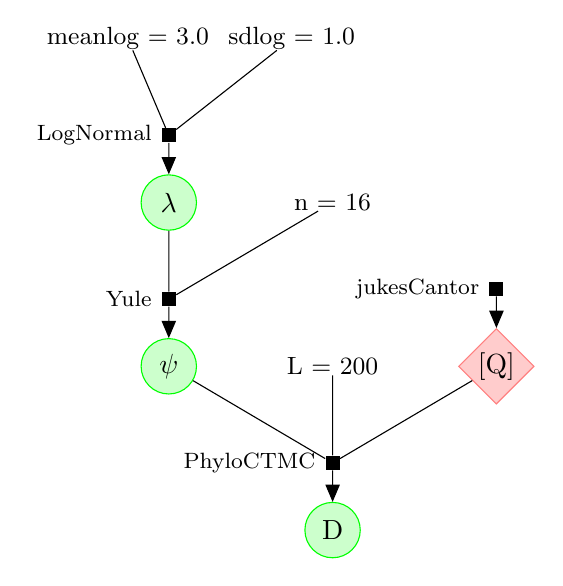
\begin{tikzpicture}[scale=0.52,
dstyle/.style={draw=blue!50,fill=blue!20},
vstyle/.style={draw=green,fill=green!20},
cstyle/.style={font=\small},
detstyle/.style={draw=red!50,fill=red!20}
]
\node[const, cstyle] at (1.0, -0.0) (602717583) {meanlog = 3.0};
\node[const, cstyle] at (5.0, -0.0) (897996787) {sdlog = 1.0};
\node[latent, vstyle] at (2.0, -4.0) (lambda) {$\lambda$};
\node[const, cstyle] at (6.0, -4.0) (2011155364) {n = 16};
\node[latent, vstyle] at (2.0, -8.0) (psi) {$\psi$};
\node[const, cstyle] at (6.0, -8.0) (1992433642) {L = 200};
\node[det, detstyle] at (10.0, -8.0) (258223775) {[Q]};
\node[latent, vstyle] at (6.0, -12.0) (D) {D};
\factor[above=of lambda] {LogNormallambda} {left:LogNormal} {} {} ; %
\factoredge {602717583, 897996787} {LogNormallambda} {lambda}; %
\factor[above=of psi] {Yulepsi} {left:Yule} {} {} ; %
\factoredge {lambda, 2011155364} {Yulepsi} {psi}; %
\factor[above=of 258223775] {jukesCantor258223775} {left:jukesCantor} {} {} ; %
\factoredge {} {jukesCantor258223775} {258223775}; %
\factor[above=of D] {PhyloCTMCD} {left:PhyloCTMC} {} {} ; %
\factoredge {1992433642, 258223775, psi} {PhyloCTMCD} {D}; %
\end{tikzpicture}}
%\end{minipage}

\item Posterior

$$P(\psi, \lambda | D) \propto P(D | \psi) P(\psi | \lambda) P(\lambda) $$

\end{enumerate}

\end{mybox}

Each of the lines in this model specification expresses how a random
variable (to the left of the tilde) is generated by a generative
distribution to the right.

The first line creates a random variable (\texttt{lambda}), that is
log-normally distributed.
The second line creates a tree (\texttt{tree}) with 16 taxa from the
Yule process with a lineage birth rate equal to \texttt{lambda}.
The third line produces a multiple sequence alignment (\texttt{D})
with a length of 200, by simulating a Jukes Cantor model of sequence
evolution down the branches of  \texttt{tree}.
As you can see, each of the random variables depends on the previous,
so this is a hierarchical model that ultimately defines a probability
distribution over sequence alignments of size $16 \times 200$.

To construct an analysis of a data set with this model we add a data block:

{\small
\begin{alltt}
data \{
  D = \textcolor{magenta!80!black}{readNexus}(\textcolor{gray}{file=}\textcolor{magenta}{"data/primate.nex"});
  L = D.\textcolor{magenta!80!black}{nchar}();
  taxa = D.\textcolor{magenta!80!black}{taxa}();
\}
model \{
  \textcolor{green}{lambda} ~ \textcolor{blue}{LogNormal}(\textcolor{gray}{meanlog=}\textcolor{magenta}{3.0}, \textcolor{gray}{sdlog=}\textcolor{magenta}{1.0});
  \textcolor{green}{tree} ~ \textcolor{blue}{Yule}(\textcolor{gray}{lambda=}\textcolor{green}{lambda}, \textcolor{gray}{taxa=}taxa);
  \textcolor{green}{D} ~ \textcolor{blue}{PhyloCTMC}(\textcolor{gray}{L=}L, \textcolor{gray}{Q=}\textcolor{magenta!80!black}{jukesCantor}(), \textcolor{gray}{tree=}\textcolor{green}{tree});
\}
\end{alltt}}

These two blocks of statements contain all the information needed to define
a Bayesian phylogenetic analysis of a multiple sequence alignment.
The data block may contain literals, and deterministic values, including those read in from a file, but not random variables or generative distributions.
The model block contains all random variables, generative distributions and boundary conditions that define the model.
If a value in the data block has the same name as a random variable in the model block, then that signifies that the data block value is an observation of the random variable with the same name.


So by assigning the alignment in file
``data/primate.nex'' to the name D in the data block we are saying that the random variable in the model named D has
been observed, and we will infer all the other random variables
(tree and lambda in this example) in the model from that observed sequence alignment.

\subsection*{Language features}

LinguaPhylo has two main components: Values (which can be either constant or random variables, and either objects or primitives) and Generators (which can be either generative distributions, deterministic functions or method calls).

\subsection*{Values}

Values in LinguaPhylo represent either random variables or constants. The type system of LinguaPhylo is open and can be extended by adding types to the Java implementation of LPhy. The types already developed include standard primitive types such as Double, Integer, String and Boolean, as well as some more complex types such as TimeTree and Alignment.

\subsection*{Primitive constants}

The simplest type of value in LinguaPhylo is a primitive constant such in the following example. The first line defines a constant named `a' with a value of `2.0'. There is no explicit statement of the type, which is simply inferred to be a Double because the literal string `2.0' has a fractional component. The second constant `b' here is a constant of type Integer because it has no decimal point or fractional component. The third constant is of primitive type Boolean, inferred by the keyword `true'. the last constant is of type String because of the double quotes surrounding the literal value.

{\singlespacing
\begin{alltt}
  a = 2.0;
  b = 2;
  c = true;
  d = "lphy";
\end{alltt}
}

\subsection*{Arrays}

The notion of primitives can be extended to arrays and to declare a constant array you can enclose comma-delimited literals in square brackets as shown below. For sequences of consecutive integers a more compact notation can be employed using the `:' to define a range. In the example below a and b represent the same constant array containing the consecutive integers from 1 to 10 inclusive.

\begin{alltt}
  a = [1, 2, 3, 4, 5, 6, 7, 8, 9, 10];
  b = 1:10;
\end{alltt}

\subsection*{Generative distributions}

A generative distribution generates a named random variable which has a value that is either an object or a primitive type. Some generative distributions have parameters which have argument labels:

{\singlespacing
\begin{alltt}
  lambda ~ LogNormal(meanlog=3.0, sdlog=1.0);
\end{alltt}
}

\subsection*{Deterministic functions}

A deterministic function generates either an object or a primitive value that is a deterministic function of its arguments. If the function has a single argument then no argument label is needed, otherwise arguments are labelled in the same way as for generative distributions. In the code below the function named hky takes two parameters with argument labels `kappa' and `freq' and deterministically produces an instantaneous rate matrix using those values.

{\singlespacing
\begin{alltt}
  Q = hky(kappa=2.0, freq=[0.2, 0.25, 0.4, 0.15]);
\end{alltt}
}

\subsection*{Vectorization}

LinguaPhylo has built-in vectorization so that any distribution or function can be called with a vectorized form of its arguments to produce multiple values from the generator. There are two vectorization patterns: IID and vectorized argument. The following code demonstrates both:

{\singlespacing
\begin{alltt}
  n = 3;
  \textcolor{green}{\(\kappa\)} ~ \textcolor{blue}{LogNormal}(\textcolor{gray}{sdlog=}\textcolor{magenta}{0.5}, \textcolor{gray}{meanlog=}\textcolor{magenta}{1.0}, \textcolor{gray}{replicates=}n);
  \textcolor{green}{\(\pi\)} ~ \textcolor{blue}{Dirichlet}(\textcolor{gray}{conc=}[\textcolor{magenta}{2.0}, \textcolor{magenta}{2.0}, \textcolor{magenta}{2.0}, \textcolor{magenta}{2.0}], \textcolor{gray}{replicates=}n);
  \textcolor{black}{Q = }\textcolor{magenta!80!black}{hky}(\textcolor{gray}{kappa=}\textcolor{green}{\(\kappa\)}, \textcolor{gray}{freq=}\textcolor{green}{\(\pi\)});

\end{alltt} 

The first two lines of this code use the IID pattern, which involves adding a replicates argument of type integer to any generative distribution. In the first line this results in a an array of iid doubles being produced from the specified log-normal distribution of length $n = 3$ instead of a single double. The second line similarly produces a 2D array of doubles representing three iid Dirichlet distributions, instead of the normal 1D array that the Dirichlet distribution would normally produce. The final line vectorises the hky funcgtion by passing arguments that are arrays of the normal argument types, resulting in the production of a 3D array representing and array of three iid HKY instantaneous rate matrices.

\subsection*{Tree generative distributions}

There are many statistical programming languages such as Stan
\cite{carpenter2017stan}, JAGS \cite{plummer2003jags} and BUGS \cite{lunn2009bugs, gilks1994language} that provide the possibility
of succinctly describing statistical models. The unique model feature of
phylogenetic analysis is the phylogenetic tree.
This is a complex high-dimensional object, part discrete, part
continuous.
There is no bijection between tree space and Euclidean space, so it
can not be treated with standard statistical distributions.
As a result specialist software is needed to perform inference \cite{hohna2016revbayes,bouckaert2019beastanalysis}.

The aim of LPhy is describe the standard phylogenetic tree
distributions succinctly and precisely, while leaving out trivial algorithmic details related to the method
of inference and the particular software employed to do the inference.

\subsubsection*{Coalescent generative distributions for time trees}

LPhy has describes a family of coalescent generative distributions
that produce TimeTrees.

The simplest model in this package is the one parameter model
constant-population size coalescent.
The generation-time-scaled population size parameter (theta) parameter determines at
what rate, per unit time, a pair of lineages coalesce, backwards in time.

\subsubsection*{Constant population size coalescent model}

In its simplest form \cite{kingman81} the coalescent model produces a
tree on a fixed number of leaves based on a population size parameter (theta):

\begin{alltt}
  g ~ Coalescent(theta=0.1, n=16);
\end{alltt}

It is also possible to give explicit taxa labels to the generative
distribution:

\begin{alltt}
  g ~ Coalescent(theta=0.1, taxa=["a", "b", "c", "d"]);
\end{alltt}

It is also possible to handle serially-sampled (time-stamped) data by
adding ages.
There are two ways to do that:

Ages without taxa names:

\begin{alltt}
  g ~ Coalescent(theta=0.1, ages=[0.0, 0.1, 0.2, 0.3]);
\end{alltt}

Ages and taxa names:

\begin{alltt}
  taxaAges = taxaAges(taxa=["a", "b", "c", "d"], ages=[0.0, 0.1, 0.2, 0.3]);
  g ~ Coalescent(theta=0.1, taxaAges=taxaAges);
\end{alltt}

\subsubsection*{Classic skyline coalescent model}

A highly parametric version of the coalescent is also possible, where
a series of theta values are provided, one for each group of consecutive coalescent intervals.
If the groupSizes are specified then each coalescent interval is given its
own population size.
The following code would generate a tree of five taxa, since there are four theta values provided:

\begin{alltt}
  g ~ SkylineCoalescent(theta=[0.1, 0.2, 0.3, 0.4]);
\end{alltt}

The theta values are indexed from the present into the past.
So the first coalescent interval (starting from the leaves)
would be generated assuming a population size parameter of 0.1, while
the last coalescent interval (culimating at the root of the tree)
would be generated from a population size parameter of 0.4.

It is also possible to add taxa and/or taxa age information:

\begin{alltt}
  taxaAges = taxaAges(taxa=["a", "b", "c", "d"], ages=[0.0, 0.1, 0.2, 0.3]);
  g ~ SkylineCoalescent(theta=[0.1, 0.2, 0.3], taxaAges=taxaAges);
\end{alltt}

This will produce a serial coalescent tree with three distinct epochs
of population size on four taxa with distinct ages.

\subsubsection*{Generalized skyline coalescent model}

The following generative distribution call will produce a tree of size
n=11 taxa, since 4+3+2+1=10= coalescent intervals.
The first four intervals will all have theta=0.1, the next three will
have theta=0.2, the next two will have theta=0.3, and the last
coalescent interval will have theta=0.4:

\begin{alltt}
  g ~ SkylineCoalescent(theta=[0.1, 0.2, 0.3, 0.4], groupSizes=[4,3,2,1]);
\end{alltt}

\subsubsection*{Structured coalescent}

A structured coalescent process takes a migration matrix (M) with
population sizes of each deme on the diagonal:
For K demes, theta is an K-tuple and the dimension of m is $K^2 -
K$. $n$ is a tuple of sample sizes, one dimension for each deme:

\begin{alltt}
  M = migrationMatrix(theta=[0.1, 0.1], m=[1.0, 1.0]);
  g ~ StructuredCoalescent(M=M, n=[15, 15]);
\end{alltt}

\subsubsection*{Multispecies coalescent}

This model allows for gene tree-species tree discordance, and is a
hierarchical model of phylogeny.
A simple multispecies coalescent model has one distribution define a
species tree, and a second distribution define a gene tree based on
the species tree:

\begin{alltt}
  S ~ Yule(lambda=5, n=4);
  theta = [0.1, 0.1, 0.1, 0.1, 0.1, 0.1, 0.1];
  g ~ MultispeciesCoalescent(theta=theta, n=[2, 2, 2, 2], S=S);
\end{alltt}

Each branch in the species tree has its own theta value.
The $n$ value describes how many individuals are represented in
the gene tree for each species.
It is a tuple of integers with length equal to the number of species
in the species tree.

\subsubsection*{Birth-death process generative distributions of trees}

The other main family of tree distributions is the birth-death-sampling generative distributions.

The simplest model in this family is the one parameter model Yule model \cite{yule1925ii}.
The birth rate (lambda) parameter determines at what rate, per unit time, each lineage bifurcates to produce two daughter lineages.
This describes a pure birth process, so that the number of lineages grows monotonically forward in time.

\subsubsection*{Yule model}

In its simplest form the Yule model has a stopping criterion based on the final number of leaves in the tree.
The following code will generate a random Yule tree with 16 leaves:

\begin{alltt}
  tree ~ Yule(lambda=1.0, n=16);
\end{alltt}

It is also possible to give explicit taxa labels to the generative distribution:

\begin{alltt}
  taxa = 1:16;
  tree ~ Yule(lambda=1.0, taxa=taxa);
\end{alltt}

or

\begin{alltt}
  taxa = ["A", "B", "C", "D"];
  tree ~ Yule(lambda=1.0, taxa=taxa);
\end{alltt}

\subsubsection*{Calibrated Yule model}

It is also possible the generate a Yule tree with a given rootAge:

\begin{alltt}
  tree ~ Yule(lambda=1.0, n=16, rootAge=10);
\end{alltt}

This is useful if you want to produce a calibrated analysis where there is a separate prior on the root age of the tree:

\begin{alltt}
  rootAge ~ LogNormal(meanlog=2.0, sdlog=1.0);
  tree ~ Yule(lambda=1.0, n=16, rootAge=rootAge);
\end{alltt}

\subsubsection*{Birth-death model}

The birth-death tree process is a generalisation of the Yule model. A second rate of extinction (mu) is added alongside
the rate of speciation (lambda). Running forward in time it is possible for the number of lineages to both grow and
shrink, and indeed for the tree process to go completely extinct.

\subsubsection*{Calibrated Birth-Death process}

A calibrated birth-death process can be describe like so:

\begin{alltt}
  tree ~ BirthDeath(lambda=2.0, mu=1.0, n=16, rootAge=10);
\end{alltt}

It is important to realise that the resulting tree will contain only the extant lineages. All extinct lineages will be
suppressed. As with the Yule model it is possible to directly specify the taxa names:

\begin{alltt}
  taxa = ["A", "B", "C", "D"];
  tree ~ BirthDeath(lambda=2.0, mu=1.0, taxa=taxa, rootAge=10);
\end{alltt}

\subsubsection*{Full birth-death process}

It is possible to generate a full birth-death tree that includes also extinct lineages using the following generative
distribution:

\begin{alltt}
  tree ~ FullBirthDeath(lambda=2.0, mu=1.0, rootAge=10);
\end{alltt}

Note that unlike the BirthDeath generative distribution, this process will generate a tree with a random number of
leaf nodes, both in terms of extinct and extant lineages. The only conditioning is on the root age.

\subsubsection*{Birth-death-sampling process}

A birth-death-sampling process adds a third parameter (rho) the probability of sampling each extant lineage. Again,
only extant lineages are leaves in the resulting tree and extinct lineages are suppressed:

\begin{alltt}
  T ~ BirthDeathSampling(lambda=2.0, mu=1.0, rho=0.5, rootAge=3);
\end{alltt}

An alternative parameterization allows specification of the diversification and turnover rates:

\begin{alltt}
  T ~ BirthDeathSampling(diversification=1.0, turnover=0.5, rho=0.5, rootAge=3);
\end{alltt}

Again it is important to note that the number of tips of the tree is a random variable, and is not conditioned on,
unlike for the BirthDeath generative distribution above.

\subsubsection*{Birth-death-serial-sampling process}

A birth-death-serial-sampling \cite{stadler2013dating} process adds a fourth parameter (psi), the rate of sampling each lineage per unit time.
Now leaves of the tree can either be extinct (psi-sampled) or extant (rho-sampled).

\begin{alltt}
  ages = [0.0,1.0,2.0,3.0,4.0];
  tree ~ BirthDeathSerialSampling(lambda=1, mu=0.5, rho=0.1, psi=1, rootAge=5, ages=ages);
\end{alltt}

In this case the number of leaves in the tree, and their ages are conditioned on, so are not random variables.


\subsection*{Models of evolutionary rates and sequence evolution}

Another key distribution necessary to perform phylogenetic inference
is the phylogenetic continuous-time Markov process and its inference
equivalent the phylogenetic likelihood \cite{felsenstein1981}.

In its simplest form the PhyloCTMC generative
distribution takes an instantaneous transition matrix (Q), a number of sites (L) and a tree:

\begin{alltt}
  tree = newick(tree="((A:0.1,B:0.1):0.2,(C:0.15,D:0.15):0.15);");
  D ~ PhyloCTMC(tree=tree, Q=jukesCantor(), L=100);
\end{alltt}

\subsection*{Molecular clock}

If the tree is not in units of substitutions per site, then it is possible to include a molecular clock rate
to scale the branches of the tree from time to substitutions per site. This example will give the same
result as the previous example, but the tree is now in units of time, so the mutation rate (mu) in units of
substitutions per site per unit time is given.

\begin{alltt}
  tree = newick(tree="((A:10,B:10):20,(C:15,D:15):15);");
  D ~ PhyloCTMC(tree=tree, Q=jukesCantor(), L=100, mu=0.01);
\end{alltt}

\subsection*{ Nucleotide substitution models}

There are a number of built in functions to construct standard nucleotide rate matrices. Some examples:

\begin{alltt}
  jc = jukesCantor();
  hky = hky(kappa=2.0, freq=[0.2, 0.25, 0.3, 0.25]);
  gtr = gtr(rates=[0.1, 0.25, 0.15, 0.15, 0.25, 0.1], freq=[0.2, 0.25, 0.3, 0.25]);
\end{alltt}

The Dirichlet prior is a natural prior for relative rates and frequencies, so a full model for GTR could
look like this:

\begin{alltt}
  pi ~ Dirichlet(conc=[3.0,3.0,3.0,3.0]); // dirichlet prior on base frequencies
  R ~ Dirichlet(conc=[1.0, 2.0, 1.0, 1.0, 2.0, 1.0]); // dirichlet prior on relative rates
  Q = gtr(freq=pi, rates=R); // construct the GTR instantaneous rate matrix
\end{alltt}

\subsection*{ Rate heterogeneity across sites}

The PhyloCTMC generative distribution takes a parameter siteRates to describe rates across sites.
For inference, a common model is the discretized Gamma distribution of site rate heterogeneity (Yang, 1994).

To match this model for simulation in LPHY do the following:

\begin{alltt}
  tree = newick(tree="((A:0.1,B:0.1):0.2,(C:0.15,D:0.15):0.15);");
  siteRates ~ G(shape=0.5, ncat=4, reps=100); // generate 100 site rates from a discretized Gamma
  D ~ PhyloCTMC(tree=tree, Q=jukesCantor(), siteRates=siteRates);
\end{alltt}

\subsection*{  Relaxed clock models (rate heterogeneity across branches) }

The PhyloCTMC generative distribution can also take an optional parameter branchRates to describe the
rates across branches:

\begin{alltt}
  tree = newick(tree="((A:0.1,B:0.1):0.2,(C:0.15,D:0.15):0.15);");
  branchRates = [0.5, 2.0, 1.0, 1.0, 2.0, 0.5];
  D ~ PhyloCTMC(L=100, Q=jukesCantor(), tree=tree, branchRates=branchRates);
\end{alltt}

\subsection*{LinguaPhylo Studio}

Along with the language definition, we also provide software to
specify and visualise models as well as simulate data from models
defined in LPhy.

This software will also provide the ability for models specified in
the LPhy language to be applied to data using standard inference tools
such as MrBayes, RevBayes, BEAST1 and BEAST2
\cite{bouckaert2014beastanalysis,DrummondBouckaert2015,bouckaert2019beastanalysis}.
This will require software that can convert an LPhy specification into
an input file that these inference engines understand.
The first such software converter is LPhyBEAST described below.

\subsection*{LPhyBEAST}

LPhyBEAST is a command-line program that takes an LPhy model
specification, and some data and produces a BEAST 2 XML input file.
It is therefore an alternative way to succinctly express and
communicate BEAST analyses.

% Results and Discussion can be combined.
\section*{Results}

\begin{itemize}
\item for evolutionary biologists
\begin{enumerate}
\item describe complex phylogenetic models succinctly and exactly
\item simulate prior distributions from these models, including arbitrary statistics
\item use model description to run inference on a real data set using LPhyBEAST
\item produce precise methods section and graphical model figure for describing analyses in published works
\end{enumerate}
\item for computational biologists
\begin{enumerate}
\item enable easy extension of the type system and generative distributions available using the plugin architecture of Lingua Phylo Studio (in Java programming language)
\item implement MCMC inference in BEAST2 for new models using LPhyBEAST and its plugin architecture
\item do well-calibrated simulation study that validate the implementation of inference framework
\end{enumerate}
\end{itemize}


\section*{Discussion}

\section*{Conclusion}

\section*{Supporting information}

% Include only the SI item label in the paragraph heading. Use the \nameref{label} command to cite SI items in the text.
\paragraph*{S1 Fig.}
\label{S1_Fig}
{\bf Bold the title sentence.} Add descriptive text after the title of the item (optional).

\paragraph*{S2 Fig.}
\label{S2_Fig}
{\bf Lorem ipsum.} Maecenas convallis mauris sit amet sem ultrices gravida. Etiam eget sapien nibh. Sed ac ipsum eget enim egestas ullamcorper nec euismod ligula. Curabitur fringilla pulvinar lectus consectetur pellentesque.

\paragraph*{S1 File.}
\label{S1_File}
{\bf Lorem ipsum.}  Maecenas convallis mauris sit amet sem ultrices gravida. Etiam eget sapien nibh. Sed ac ipsum eget enim egestas ullamcorper nec euismod ligula. Curabitur fringilla pulvinar lectus consectetur pellentesque.

\paragraph*{S1 Video.}
\label{S1_Video}
{\bf Lorem ipsum.}  Maecenas convallis mauris sit amet sem ultrices gravida. Etiam eget sapien nibh. Sed ac ipsum eget enim egestas ullamcorper nec euismod ligula. Curabitur fringilla pulvinar lectus consectetur pellentesque.

\paragraph*{S1 Appendix.}
\label{S1_Appendix}
{\bf Lorem ipsum.} Maecenas convallis mauris sit amet sem ultrices gravida. Etiam eget sapien nibh. Sed ac ipsum eget enim egestas ullamcorper nec euismod ligula. Curabitur fringilla pulvinar lectus consectetur pellentesque.

\paragraph*{S1 Table.}
\label{S1_Table}
{\bf Lorem ipsum.} Maecenas convallis mauris sit amet sem ultrices gravida. Etiam eget sapien nibh. Sed ac ipsum eget enim egestas ullamcorper nec euismod ligula. Curabitur fringilla pulvinar lectus consectetur pellentesque.

\section*{Acknowledgments}
Cras egestas velit mauris, eu mollis turpis pellentesque sit amet. Interdum et malesuada fames ac ante ipsum primis in faucibus. Nam id pretium nisi. Sed ac quam id nisi malesuada congue. Sed interdum aliquet augue, at pellentesque quam rhoncus vitae.

\nolinenumbers

% Either type in your references using
% \begin{thebibliography}{}
% \bibitem{}
% Text
% \end{thebibliography}
%
% or
%
% Compile your BiBTeX database using our plos2015.bst
% style file and paste the contents of your .bbl file
% here. See http://journals.plos.org/plosone/s/latex for 
% step-by-step instructions.
% 
\bibliography{linguaPhylo}



\end{document}

